\subsection{Airfoil Analysis}
The desired cruise conditions for the aircraft fall within transonic speed regime.  This provides favorable conditions for the sizing analysis but results in an increase in wave drag force.

\begin{wrapfigure}{r}{0.5\textwidth}
    \vspace{-0.25in}
    \centering
    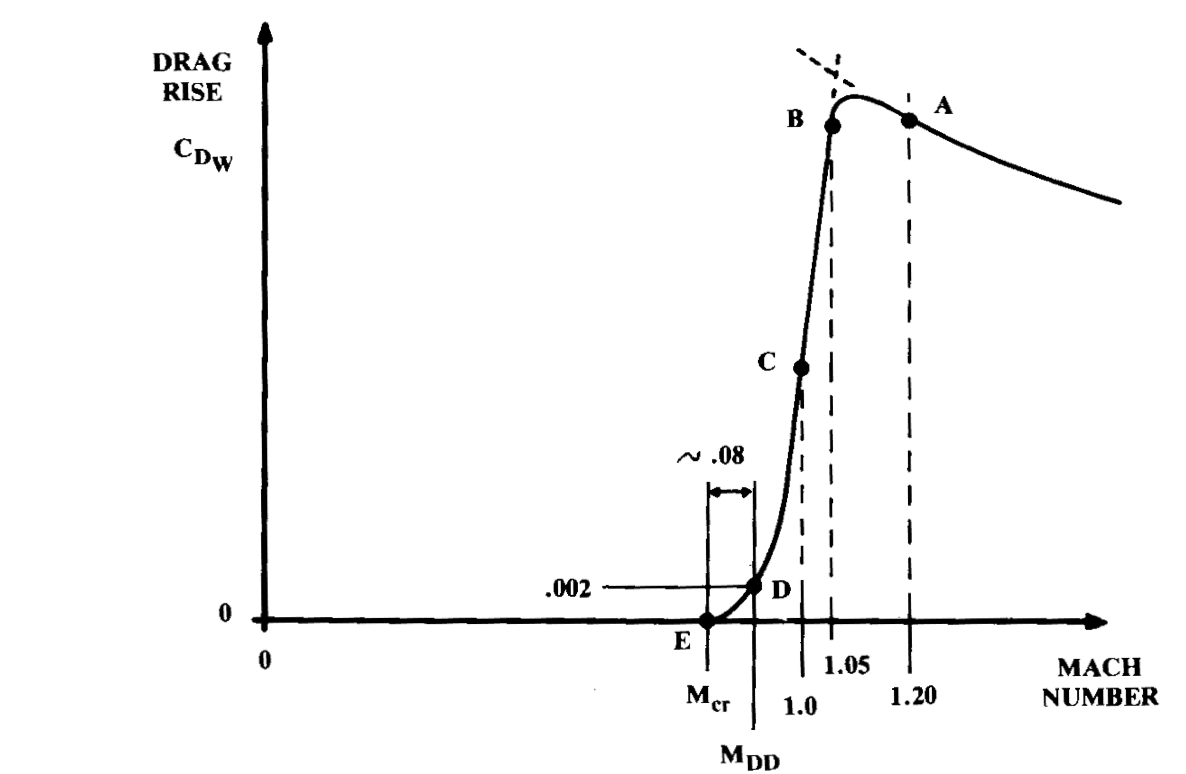
\includegraphics[width=0.5\textwidth]{Photos/wavedragduetotransonic.png}
    \caption{Wave Drag due to Transonic Airspeed\\{\small From Raymer Fig. 12.29\cite{raymer}}}
    \label{fig:transonic}
    \vspace{-0.5in}
\end{wrapfigure}

As shown above in Figure \ref{fig:transonic}, there is an increase in wave drag as the aircraft passes into the transonic regime.  Therefore, a selection of supercritical airfoils and wing sweep of no less than $30\degree$ is proposed in mitigation of the above trend.  To properly predict and quantify the wave drag for aerodynamic analysis on the airfoil and wing design, \textit{Method B} from Vargas\cite{vargas} shall be included in the part-by-part drag buildup.

\subsection{Wing Design}
Initial assumptions were made for the aspect ratio of the wing design based on comparable aircraft such as the Boeing 777-300 and Boeing 787.  Consequently, a range of $\AR \in [8,12]$ was initially set.  A wing area of $5,000 \text{ ft}^2$ was recommended from performance analysis.  

The wing dimensions are shown to the below in Table \ref{tab:wingsizing}.

\begin{table}[!h]
    \centering
    \caption{Wing Dimensions}
    \begin{tabular}{|c|c|c|} \toprule
        \multicolumn{3}{c}{\textbf{\textcolor{cobalt}{Main Wing}}} \\ \midrule
        \textbf{Description} & \textbf{\#} & \textbf{Units} \\ \hline \hline
        \AR & 9 & $\sim$ \\ \hline
        b (\textit{span}) & 212 & ft \\ \hline 
        $S_{\text{wing}}$ (\textit{area}) & 5,000 & ft$^2$ \\ \hline
        c/4 Sweep & $30$ & degree \\ \hline
        Taper & 0.18 & $\sim$ \\ \hline
        Chord Root & 479.39 & in \\ \hline
        Chord Tip & 86.291 & in \\ \hline
        Mean Aerodynamic Chord & 328.37 & in \\ \bottomrule
    \end{tabular}
    \label{tab:wingsizing}
\end{table}

\clearpage

\subsection{Drag Buildup}
The Drag for Sam Mark I. is built up part-by-part by separating the fuselage, wings, empennage, and other protuberances and calculating the following seven key forms of drag, shown in Equation \ref{eqn:drag_general}:
\begin{equation}\label{eqn:drag_general}
    C_D = C_{D,0} + C_{D,i} + C_{D,W_{NL}} + C_{D,W_{L}} + C_{D_{EXCR}} + \Delta C_{D_{Re}} + C_{D,trim}
\end{equation}


\subsection{High-Lift Systems}
The mission profile requires high lift devices to improve the aircraft stability during the take-off and landing segments.  Therefore, high-lift systems such as leading edge slats and trailing edge Fowler flaps are included in the structure of the wing.

\subsection{Future Progress}
The following topics will be further investigated for the Preliminary Design Report:
\begin{itemize}
    \item Complete Drag Buildup
    \item High lift devices during Take-off/Landing, Lift-Drag Polars, and Impact of flaps and slats on aircraft stability
    \item XFLR5 Analysis of Supercritical Airfoils to determine desired airfoil
    \item Wing geometry with airfoil design
    \item Analyze 
\end{itemize}

\hl{Josh: complete this}

% Will talk about supercritical airfoil analysis, run-through preliminary XFLR5 data, and general drag buildup. - Josh

\textcolor{red}{
\begin{itemize}
    \item Discuss wing design, including reasoning. \checkmark JJ
    \item Discuss high-lift system, including reasoning. \checkmark JJ
    \item Discuss drag buildup (tabulated) used to support sizing analysis. \checkmark JJ
    \item Discuss future work. X
    \item AIAA: Important aerodynamic characteristics and aerodynamic performance for key mission
    segments and requirements (shared w/ aero) N/A for now \checkmark
\end{itemize}}